{\bfseries
	Pour cette première partie, aucune justification n'est demandée et une seule réponse est possible par question.

	Pour chaque question, reportez son numéro sur votre copie et indiquez votre réponse.}

Une réponse fausse ou l'absence de réponse n'enlève aucun point.

\subsection*{Question 1}
Pour tout nombre réel $x$, \quad $(5x-2)^{2}$ \quad est égal à :

\begin{tblr}{colspec = {*4{X}}}
	\textbf{A.}\quad {$5x^{2}-4$}&
	\textbf{B.}\quad {$(5x-2)(5x+2)$}&
	\textbf{C.}\quad {$25x^{2}+4$}&
	\textbf{D.}\quad {$25x^{2}-20x+4$}\\
\end{tblr}

\subsection*{Question 2}
Le nombre \quad $\dfrac{1}{4}\times\dfrac{8}{5}-\dfrac{1}{5}$ \quad est égal à :

\begin{tblr}{colspec = {*4{X}}}
	\textbf{A.}\quad {$\dfrac{1}{4}$}&
	\textbf{B.}\quad {$\dfrac{7}{20}$}&
	\textbf{C.}\quad {$\dfrac{19}{15}$}&
	\textbf{D.}\quad {$\dfrac{1}{5}$}\\
\end{tblr}

\subsection*{Question 3}
Multiplier une quantité par $\dfrac{3}{4}$ c'est lui appliquer :

\begin{tblr}{colspec = {*2{X}}}
	\textbf{A.}\quad une baisse de 25\,\% ;&
	\textbf{B.}\quad une hausse de 25\,\% ;\\
	\textbf{C.}\quad une baisse de 75\,\% ;&
	\textbf{D.}\quad une hausse de 75\,\%.\\
\end{tblr}

\subsection*{Question 4}
Dans l'ensemble des nombres réels, l'équation \quad $(2x-4)(-3x+3)=0$\quad a pour ensemble de solutions :

\begin{tblr}{colspec = {*4{X}}}
	\textbf{A.}\quad {$S=\{2~;~-1\}$}&
	\textbf{B.}\quad {$S=\{2~;~1\}$}&
	\textbf{C.}\quad {$S=[2~;~-1]$}&
	\textbf{D.}\quad {$S=[2~;~1]$}\\
\end{tblr}

\subsection*{Question 5}
Le prix d'un article a subi une baisse de 50\,\% en 2024 puis ensuite il augmente de 50\,\% en 2025.

Entre le début 2024 et la fin 2025, le prix de l'article :

\begin{tblr}{colspec = {*2{X}}}
	\textbf{A.}\quad n'a pas changé ;&
	\textbf{B.}\quad a augmenté de 5\,\% ;\\
	\textbf{C.}\quad a diminué de 25\,\% ;&
	\textbf{D.}\quad a augmenté de 25\,\%.\\
\end{tblr}

\subsection*{Question 6}
\begin{minipage}{0.55\linewidth}
	On considère la fonction affine $f$ dont la représentation graphique, donnée ci-contre, est la droite passant par les points A$(3 ; -1)$ et B$(1;3)$.

	\medskip

	Pour tout réel $x$ :

	\begin{tblr}{colspec = {*2{X}}}
		\textbf{A.}\quad {$f(x)=5x+2{,}5$}&
		\textbf{B.}\quad {$f(x)=-2x+5$}\\
		\textbf{C.}\quad {$f(x)=-2{,}5x+5$}&
		\textbf{D.}\quad {$f(x)=-0{,}5x+5$}\\
	\end{tblr}
\end{minipage}\hfill
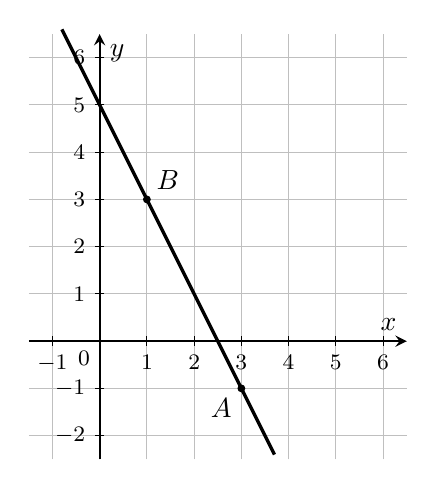
\begin{tikzpicture}[scale=0.6, baseline={(current bounding box.center)}]
	\draw[gray!50, line width=0.4pt] (-1.5,-2.5) grid (6.5,6.5);
	\draw[line width=0.8pt,->,>=stealth] (-1.5,0) -- (6.5,0) node[above left]{$x$};
	\draw[line width=0.8pt,->,>=stealth] (0,-2.5) -- (0,6.5) node[below right]{$y$};
	\foreach \x in {-1,1,2,3,4,5,6}
	\draw (\x,0.1) -- (\x,-0.1) node[below, font=\footnotesize]{$\np{\x}$};
	\foreach \y in {-2,-1,1,2,3,4,5,6}
	\draw (0.1,\y) -- (-0.1,\y) node[left, font=\footnotesize]{$\np{\y}$};
	\node[below left, font=\footnotesize] at (0,0) {$0$};
	\draw[line width=1.2pt] (-0.8,6.6) -- (3.7,-2.4);
	\filldraw (1,3) circle (2pt) node[above right]{$B$};
	\filldraw (3,-1) circle (2pt) node[below left]{$A$};
\end{tikzpicture}\hfill~

\subsection*{Question 7}
\begin{center}
	\begin{tblr}{colspec={|c|X[c,1cm]|X[c,1cm]|X[c,1cm]|}, hlines}
		\textbf{Notes} & 18 & 11 & 16 \\
		\textbf{Coefficients} & 1 & 2 & 1 \\
	\end{tblr}
\end{center}

La moyenne coefficientée des trois notes ci-dessus est égale à :

\begin{tblr}{colspec = {*4{X}}}
	\textbf{A.}\quad {$15$}&
	\textbf{B.}\quad {$14{,}5$}&
	\textbf{C.}\quad {$14$}&
	\textbf{D.}\quad {$13{,}5$}\\
\end{tblr}

\subsection*{Question 8}
Un salarié a réalisé 6,4 heures supplémentaires. Cela correspond à :

\begin{tblr}{colspec = {*2{X}}}
	\textbf{A.}\quad 6 heures et 20 minutes&
	\textbf{B.}\quad 640 minutes\\
	\textbf{C.}\quad 6 heures et 40 minutes&
	\textbf{D.}\quad 6 heures et 24 minutes\\
\end{tblr}
